\chapter{The pseudo-spectral method} \label{sec_pseudspec}
The idea behind the pseudo-spectral method is first to transform
the evolution equations to Fourier (spectral) space, i.e.\ in our
example to use the eigenfunctions of the Laplacian as basis of the
space of all solutions and to project the full equations onto this basis,
see e.g.\ \cite{canutoetal1988}. Second to calculate products of functions
(non-linear terms) in the physical space and transform them back
to Fourier space to reduce the number of multiplications necessary,
which otherwise makes the spectral method computationally prohibitively
expensive for problems with a large numbers of Fourier modes. This idea
goes back to \cite{kreissandoliger1972}. More details on the
pseudospectral method can be found, e.g.\ in \cite{orszag1972}
and \cite{fornberg1987}.

\section{The discrete Fourier transform}
\label{ssec_evolfourier}
Starting point for the set of basis functions are the Fourier modes 
$F(k_{x},k_{y} \ | \ x,y)$ which are the eigenmodes of the Laplacian 
on the fluid domain considered (short notation 
$F(\mathbf{k} \ | \ \mathbf{x})$ with 
$\mathbf{k} = (k_{x},k_{y})$ and $\mathbf{x} = (x,y)$).  
We start with a doubly periodic fluid domain (default in QUAD). 
In this case the eigenmodes of the Laplacian are given by
\begin{equation} \label{eq_defFkxky}
  F(\mathbf{k} \ | \ \mathbf{x}) 
   = 
 \exp \left[ i  \left(k_{x} x + k_{y} y \right) \right]
   = 
 \exp \left[ i k_{x} x \right] \ 
 \exp \left[ i k_{y} y \right],
\end{equation}
and satisfy the eigenvalue equation
\begin{equation} \label{eq_eigFkxky}
 \Delta \ F(\mathbf{k} \ | \ \mathbf{x})
   =
  - \left( k_{x}^{2} + k_{y}^{2} \right) \ 
    F(\mathbf{k} \ | \ \mathbf{x}),
\end{equation}
with $k_{x} = n \ 2 \pi/X$ and $k_{y} = m \ 2 \pi/Y$ for 
$n,m \in [0,\pm 1, \pm 2,\ \dots \ ]$. As can be seen form equation 
(\ref{eq_defFkxky}) the eigenmodes of the Laplacian on the 
two-dimensional fluid domain 
$F(\mathbf{k} \ | \ \mathbf{x}) = F(k_{x} \ | \ x) \ F(k_{y} \ | \ y)$
can be separated into a product of the eigenmodes of the 
1-dimensional Laplacian. For more general domains
as circular discs, annuli or the surface of spheres as well as 
for more general boundary conditions, i.e. for fluid domains with walls 
one has to choose other systems of basis functions, 
see e.g.\ \cite{canutoetal1988}.

Taking $L_{x} = X/2 \pi$ and $L_{y} = Y/ 2 \pi$ in $x$ and $y$-direction 
as horizontal length scales and introducing the non-dimensional variables
$\bar{x} = x/L_{x}$, $\bar{y} = y/L_{y}$, $\bar{k}_{x} = k_{x} L_{x}$ 
and $\bar{k}_{y} = k_{y} L_{y}$ the non-dimensional eigenvalue equation
\begin{equation} \label{eq_ndeigFkxkyLxLy}
 \left[ 
  \frac{\partial^{2}}{\partial \bar{x}^{2}} 
   +
  \frac{\partial^{2}}{r^{2} \partial \bar{y}^{2}} 
 \right] \ 
  F(\mathbf{\bar{k}} \ | \ \mathbf{\bar{x}})
   = 
  - \left( \bar{k}_{x}^{2} + \frac{\bar{k}_{y}^{2}}{r^{2}} \right)
  F(\mathbf{\bar{k}} \ | \ \mathbf{\bar{x}}),
\end{equation}
with the aspect ratio of the fluid domain $r = L_{y}/L_{y} = Y/X$,
the wave number vector $\mathbf{\bar{k}} = (\bar{k}_{x},\bar{k}_{y})$, 
where $\bar{k}_{x} = \bar{k}_{y} = 0, \pm 1, \pm 2, \ \dots \ $ and the
coordinate vector $\mathbf{\bar{x}} = (\bar{x},\bar{y})$, where 
$\bar{x},\bar{y} \in [0 \ \ 2\pi]$.
Such an approach leads to a rescaled Laplacian and is appropriate 
in particular for physical problems with a strong horizontal 
anisotropy.

Introducing a single horizontal length scale as for example 
$L = L_{x} = X/2 \pi$ instead we get the non-dimensional variables 
$\bar{x} = x/L$, $\bar{y} = y/L$, $\bar{k}_{x} = k_{x} L = n$ and 
$\bar{k}_{y}/r = k_{y} L/r = m/r$. The non-dimensional eigenvalue 
equation now reads
\begin{equation} \label{eq_ndeigFkxkyL}
 \left[ 
  \frac{\partial^{2}}{\partial \bar{x}^{2}} 
   +
  \frac{\partial^{2}}{\partial \bar{y}^{2}} 
 \right] \ 
  F(\mathbf{\bar{k}} \ | \ \mathbf{\bar{x}})
   = 
  - \left( \bar{k}_{x}^{2} + \frac{\bar{k}_{y}^{2}}{r^{2}} \right)
  F(\mathbf{\bar{k}} \ | \ \mathbf{\bar{x}}),
\end{equation}
with the aspect ratio of the fluid domain $r$ defined above, 
the wave number vector $\mathbf{\bar{k}} = (\bar{k}_{x},\bar{k}_{y}/r)$, 
where $\bar{k}_{x} = \bar{k}_{y} = 0, \pm 1, \pm 2, \ \dots \ $ and
the coordinate vector $\mathbf{\bar{x}} = (\bar{x},\bar{y})$, where
$\bar{x} \in [0 \ 2 \pi]$ and $\bar{y} \in [0 \ r 2 \pi]$. 
In QUAD we use a single horizontal length scale 
keeping in mind that this choice is not optimal for problems 
with a strong horizontal anisotropy. In the special case of a square domain 
(default case in QUAD) we have $r = 1$.
From now on we use, if not otherwise stated, the non-dimensional form and 
omit overbars. 

Using the Fourier modes $F(\mathbf{k} \ | \ \mathbf{x})$ we can expand all 
fields $g(x,y,t)$ on the fluid domain into a Fourier series
\begin{equation} \label{eq_fourierser}
  g(x,y,t) 
   =  
  \sum_{k_{x} = -\infty}^{\infty} \ \sum_{k_{y} = -\infty}^{\infty} \ 
   \hat{g}(k_{x},k_{y},t) \ 
   \exp
   \left[ 
     i \left(k_{x} x + \frac{k_{y}}{r} y \right)
   \right],
\end{equation}
where $\hat{g}(k_{x},k_{y},t)$ are the Fourier coefficients of 
$g(x,y,t)$ which live on the space of wave numbers $(k_{x},k_{y})$.
Since $g(x,y,t)$ are real fields, the Fourier modes $\hat{g}(k_{x},k_{y},t)$
have the symmetry property that
\begin{equation} \label{eq_symfourier}
  \hat{g}(-k_{x},-k_{y},t)  = \hat{g}^{\ast}(k_{x},k_{y},t),
\end{equation}
where $g^{\ast}$ is the complex conjugate of $g$. The Fourier
coefficients $\hat{g}(k_{x},k_{y},t)$ are obtained by the integral
\begin{equation} \label{eq_fourierintndim}
  \hat{g}(k_{x},k_{y},t)
   = 
  \frac{1}{r} \frac{1}{4 \pi^{2}} 
   \int_{0}^{2 \pi} \int_{0}^{r 2 \pi}
   \exp  
   \left[ 
    -i \left(k_{x} x + \frac{k_{y}}{r} y \right)
   \right] \
   g(x,y,t) \ 
dx dy.
\end{equation}
This continous finite Fourier integral is derived from the
dimensional integral 
\begin{equation} \label{eq_fourierint}
  \hat{g}(k_{x},k_{y},t)
   =
  \frac{1}{XY} \int_{0}^{X} \int_{0}^{Y}
   \exp
   \left[
    -i \left(k_{x} x + k_{y} y \right)
   \right] \
   g(x,y,t) \
dx dy,
\end{equation}
where $x$,$y$,$k_{x}$ and $k_{y}$ are the dimensional variables.

To use the Fourier transform in numerical schemes to solve the evolution
equation of fluids we have to approximate the continous finite Fourier integral
(\ref{eq_fourierintndim}) and the infinite Fourier series
(\ref{eq_fourierser}).

We start by discretizing the physical space into $N$ grid points in
$x$-direction and $M$ grid points in $y$-direction. On the discretized
grid of the physical space the continuous finite Fourier integral
(\ref{eq_fourierintndim}) reduces to the double sum
\begin{equation} \label{eq_fourierintprox}
   \hat{g}(k_{x},k_{y},t)
    = 
   \frac{1}{N M} 
   \sum_{n = 0}^{N-1} \sum_{m=0}^{M-1} \
    \exp 
     \left[-i    
      \left(
       k_{x} x_{n} + \frac{k_{y}}{r} y_{m}
      \right)
     \right]
     g(x_{n},y_{m},t),
\end{equation}
where we use the approximations $dx = \Delta x =2\pi/N$, 
$dy = \Delta y = r 2\pi/M $, $x_{n} = n \ \Delta x$ 
and $y_{m} = m \ \Delta y$ with $n \in [0,1,\ \dots \ ,N-1]$ and
$m \in [0,1,\ \dots \,M-1]$. The aspect ratio of the grid cell 
is given by $\Delta x/\Delta y = M/N \ 1/r$. For $r = M/N$ 
the grid cells are squares (default in QUAD $M=N$ and $r=1$).
 
Next we truncate the infinite Fourier series (\ref{eq_fourierser}) 
at wave numbers such that all modes with a higher spatial frequency 
(wave mumber) than the grid in physical space are omitted otherwise
we would have an oversampling. The result is the finite sum
\begin{equation} \label{eq_fouriersertrun}
  g(x_{n},y_{m},t) 
   =  
  \sum_{k_{x} = -\frac{N}{2}+1}^{\frac{N}{2}} \ 
  \sum_{k_{y} = -\frac{M}{2}+1}^{\frac{M}{2}} \
   \exp
   \left[ 
    i \left(k_{x} x_{n} + \frac{k_{y}}{r} y_{m} \right)
   \right] \
   \hat{g}(k_{x},k_{y},t).
\end{equation}
On the discretized grid in the physical space the modes with wave numbers 
$(k_{x},k_{y}) = (-N/2,-M/2)$ and $(k_{x},k_{y}) = (N/2,M/2)$ are 
identical. We omitted the mode $(k_{x},k_{y}) = (-N/2,-M/2)$.

Using the definitions of $x_{n} = 2 \pi \ n/N$ and $y_{m} = r 2 \pi \ m/M$ 
we can write equation (\ref{eq_fourierintprox}) in discretized form as
\begin{equation} \label{eq_fourierintdisc}
  \hat{g}(k_{x},k_{y},t)
   = 
  \frac{1}{NM} 
   \sum_{n = 0}^{N-1}
    \sum_{m = 0}^{M-1}
     \exp 
      \left[
       -i 2 \pi 
        \left( 
         \frac{k_{x} n}{N} + \frac{k_{y} m}{M}
        \right)
      \right]
      \ g(x_{n},y_{m},t)
\end{equation}
and equation (\ref{eq_fouriersertrun}) as
\begin{equation} \label{eq_fourierserdisc}
  g(x_{n},y_{m},t)
   = 
   \sum_{k_{x}= -\frac{N}{2}+1}^{\frac{N}{2}}
    \ 
    \sum_{k_{y}= -\frac{M}{2}+1}^{\frac{M}{2}}
     \exp 
      \left[ 
        i 2 \pi 
        \left( 
         \frac{k_{x} n}{N} + \frac{k_{y} m}{M}
        \right) 
      \right]
    \hat{g}(k_{x},k_{y},t).
\end{equation}
By a shift of the wave numbers $k_{x}$ and $k_{y}$ corresponding to a rotation 
in the complex plane the double sum (\ref{eq_fourierserdisc}) can be written
equivalently in the form
\begin{equation} \label{eq_fourierserdiscshift}
  g(x_{n},y_{m},t)
   = 
   \sum_{k_{x}= 0}^{N-1}
    \ 
    \sum_{k_{y}= 0}^{M-1}
     \exp 
      \left[ 
        i 2 \pi 
        \left( 
         \frac{k_{x} n}{N} + \frac{k_{y} m}{M}
        \right) 
      \right]
    \hat{g}(k_{x},k_{y},t).
\end{equation}
Relation (\ref{eq_fourierintdisc}) defines the discrete $2$-D
forward Fourier transform $\mathcal{F}_{NM}$ and relation 
(\ref{eq_fourierserdiscshift}) the discrete $2$-D inverse Fourier 
transform $\mathcal{F}^{-1}_{MN}$ respectively. One can decompose the 
$2$-D transformations $\mathcal{F}_{NM}$ and $\mathcal{F}^{-1}_{MN}$ 
into two consecutive $1$-D Fourier transformations $\mathcal{F}_{N}$, 
$\mathcal{F}_{M}$ and $\mathcal{F}^{-1}_{M}$, $\mathcal{F}^{-1}_{N}$. 

The forward Fourier transform can be decomposed as follows
\begin{equation} \label{eq_forwardfourier_2D1D}
  \hat{g}(k_{x},k_{y},t) 
    = 
  \frac{1}{N} \sum_{n=0}^{N-1} 
     \exp 
      \left( 
        - i 2 \pi \frac{k_{x} n}{N}
      \right)
  \left[
   \frac{1}{M} \sum_{m=0}^{M-1} 
      \exp 
       \left( 
         - i 2 \pi \frac{k_{y} m}{M}
       \right)
   g(x_{n},y_{m},t) 
  \right]
\end{equation}
or using operators $\hat{g} = \mathcal{F}_{NM} \ g 
= \mathcal{F}_{N} \mathcal{F}_{M} g$, where the operators 
$\mathcal{F}_{N}$ and $\mathcal{F}_{M}$ have the matrix 
representation
\begin{equation} \label{eq_forwardfourier_1D}
  \mathcal{F}_{N} = 
   \frac{1}{N} \ 
   \left(
     exp \left[-i 2 \pi \frac{k_{x} n}{N} \right]
   \right)_{k_{x},n \in [0,N-1]}
   \ \ \mbox{and} \ \ 
  \mathcal{F}_{M} = 
   \frac{1}{M} \ 
   \left(
     exp \left[-i 2 \pi \frac{k_{y} m}{M} \right]
   \right)_{k_{y},m \in [0,M-1]}
\end{equation}
For the inverse Fourier transform we get the decomposition
\begin{equation} \label{eq_inversefourier_2D1D}
  g(x_{n},y_{m},t)
    = 
  \sum_{k_{y}=0}^{M-1}
     \exp
      \left( 
          i 2 \pi \frac{k_{y} m}{M}
      \right)
  \left[
   \sum_{k_{x}=0}^{N-1} 
      \exp 
       \left( 
          i 2 \pi \frac{k_{x} n}{N}
       \right)
   \hat{g}(k_{x},k_{y},t)
  \right],
\end{equation}
which using operators can be written as 
$g=\mathcal{F}^{-1}_{MN}=\mathcal{F}^{-1}_{M} \mathcal{F}^{-1}_{N} \hat{g}$, 
where the operators $\mathcal{F}^{-1}_{N}$ and $\mathcal{F}^{-1}_{M}$ 
have the matrix representation
\begin{equation} \label{eq_inversefourier_1D}
  \mathcal{F}^{-1}_{N} = 
   \left(
     exp \left[i 2 \pi \frac{k_{x} n}{N} \right]
   \right)_{n,k_{x} \in [0,N-1]}
   \ \ \mbox{and} \ \ 
  \mathcal{F}^{-1}_{M} = 
   \left(
     exp \left[i 2 \pi \frac{k_{y} m}{M} \right]
   \right)_{m,k_{y} \in [0,M-1]}.
\end{equation}
Using as basic unit the exponent $\omega = \exp \left[-i 2 \pi/N \right]$
we can represent the one-dimensional discrete forward Fourier transform
$\mathcal{F}_{N}$ for a vector of length $N$ as
\begin{equation} \label{eq_forwardfourier_1D_matrix}
 \mathcal{F}_{N}
  =
 \frac{1}{N} \ 
 \left(
  \begin{array}{ccccc}
    1 &    1         &     1           & \dots & 1
   \\
    1 & \omega       & \omega^{2}      & \dots & \omega^{N-1}
   \\
    . &    .         &     .           &       & . 
   \\
    . &    .         &     .           &       & .
   \\
    . &    .         &     .           &       & .
   \\
    1 & \omega^{N-1} & \omega^{2(N-1)} & \dots & \omega^{(N-1)^{2}}
  \end{array}
 \right). 
\end{equation}
The inverse Fourier transform $\mathcal{F}^{-1}_{N}$ is given by the 
matrix ({\ref{eq_forwardfourier_1D_matrix}}) without the factor
$1/N$, where $\omega$ is replaced by the complex conjugate 
$\bar{\omega} = \exp \left[i 2 \pi/N \right]$. The representation of 
the Fourier matrices for small $N$ are the building 
blocks of the fast Fourier transform introduced in section (\ref{sec_fft}).   
For $N = 2$, $N = 3$ and $N = 4$ we get
\begin{equation} \label{eq_F2F3}
 \mathcal{F}_{2}
  =
 \frac{1}{2}
 \left(
  \begin{array}{cr}
     1  &  1 
        \\
     1  &  -1 
  \end{array}
 \right),
 \ \ 
 \mathcal{F}_{3}
  =
 \frac{1}{3}
 \left(
  \begin{array}{ccc}
     1    &    1         &    1
              \\
     1    & \omega       &  \bar{\omega}
              \\
     1    & \bar{\omega} &  \omega 
  \end{array}
 \right)
\ \ \ \mbox{and} \ \ \ 
 \mathcal{F}_{4}
  =
 \frac{1}{4}
 \left(
  \begin{array}{crrr}
   1   & 1   &  1  &  1
        \\
   1   & -i  & -1  &  i
        \\
   1   & -1  &  1  & -1
        \\
   1   &  i  & -1  & -i 
  \end{array}
 \right),
\end{equation}
with $\omega = -\exp (i \pi/3)=-[\cos(\pi/3)+i \ \sin(\pi/3)]$. For $N=8$ 
the representation reads     
\begin{equation} \label{eq_F4F8}
 \mathcal{F}_{8}
  =
 \frac{1}{8}
 \left(
  \begin{array}{crrrrrrr}
   1& 1       & 1& 1        & 1&     1   & 1& 1
                                           \\
   1& \omega  &-i&-i\omega  &-1& -\omega & i& i\omega 
                                           \\
   1&-i       &-1& i        & 1& -i      &-1& i
                                           \\ 
   1&-i\omega & i& \omega   &-1&  i\omega&-i&-i\omega
                                           \\  
   1&-1       & 1&-1        & 1& -1      & 1&-1
                                           \\ 
   1&-\omega  &-i& i\omega  &-1&   \omega& i&-i\omega 
                                           \\ 
   1& i       &-1&-i        & 1&  i      &-1&-i 
                                           \\ 
   1&\omega   & i&-i\omega  &-1& -i\omega&-i& \omega 
  \end{array}
 \right),
\end{equation}
with $\omega = \exp(-i \pi /4) = \sqrt{0.5} \ [1-i]$. Making
full use of the information hidden in the structure of the 
Fourier matrices one can reduce the number of multiplications
needed to carry out the Fourier transform from order 
{\it O}($N^2$) to order {\it O}($N \log N$), which makes a 
big difference for large $N$, see section \ref{sec_fft}. 

\section{Fast Fourier Transform} \label{sec_fft}
Rearranging the rows of a Fourier matrix $\mathcal{F}_{N}$
by collecting even and odd rows (assuming even $N$) we
can express $\mathcal{F}_N$ in terms of $\mathcal{F}_{N/2}$. 
One gets
\begin{equation}  \label{eq_FNFNr2}
 \mathcal{F}_{N} \ g_{N} 
  =
 \left(
  \begin{array}{cr}
   I_{N/2} &  D_{N/2}
           \\
   I_{N/2} & -D_{N/2}
  \end{array}
 \right)
 \left(
  \begin{array}{cr}
   \mathcal{F}_{N/2} &     0
           \\
        0            & \mathcal{F}_{N/2}
  \end{array}
 \right)
 \left(     
  \begin{array}{c}
   g_{N/2}^{e}
    \\
   g_{N/2}^{o}
  \end{array} 
 \right),
\end{equation} 
where $g^{e}_{N/2}$ and $g^{o}_{N/2}$ are the even and odd
components of the vector $g_{N}$. Moreover $\mathcal{F}_{N/2}$ 
is the Fourier transform of size $N/2$, $I_{N/2}$ the identity 
matrix of size $N/2$ and $D_{N/2}$ the diagonal matrix 
$D_{N/2} =  diag(1,\omega_{N},\ \dots \ , \omega_{N}^{N/2 - 1})$,
with $\omega_{N} = \exp ( -i 2 \pi / N )$. Transforming the
expression (\ref{eq_FNFNr2}) further we can write
\begin{equation}  \label{eq_FNFNr2_01}
 \mathcal{F}_{N} \ g_{N} 
  =
 \left(
  \begin{array}{cr}
   I_{N/2} &  I_{N/2}
           \\
   I_{N/2} & -I_{N/2}
  \end{array}
 \right)
 \left(
  \begin{array}{cr}
   I_{N/2} &     0
          \\
      0    &   D_{N/2}
  \end{array}
 \right)
 \left(
  \begin{array}{cr}
   \mathcal{F}_{N/2} &     0
           \\
        0            & \mathcal{F}_{N/2}
  \end{array}
 \right)
  \ P_{N}^{2} \ g_{N}
\end{equation} 
where $P_{N}^{2}$ is a permutation matrix reordering the 
vector components into $2$ blocks (even and odd). Since
the Fourier operators $\mathcal{F}_{N}$ are symmetric we can
write       


\begin{equation} \label{eq_FNFNr2_02} 
 \mathcal{F}_{N} \ g_{N} 
   = 
 \left[ \mathcal{F}_{2} \otimes I_{N/2} \right] \ 
 diag(I_{N/2},D_{N/2})  \ 
 \left[ I_{2} \otimes \mathcal{F}_{N/2} \right] \
 P_{N}^{2} \ g_{N},
\end{equation}

Taking $N=8$ as example.



\section{Evolution equations in Fourier space}
\label{ssec_evolfourier}
The basic advantage of the Fourier representation is that
differential operators as $\partial_{x}$,
$\partial_{y}$, $\partial_{x} \partial_{y}$, $\nabla$, $\Delta$
are transformed to simple multiplication operators
$i k_{x}$, $i k_{y}/r$, $- k_{x} k_{y}/r$ ,$(i k_{x},i k_{y}/r)$, 
$-(k_{x}^{2} + k_{y}^{2}/r^{2})$ in spectral space with $i = \sqrt{-1}$.
Differential equations in physical space are thus reduced to algebraic 
equations in spectral space.

In the Fourier space it is now straight forward to determine
the stream function $\hat{\psi}(k_{x},k_{y},t)$ and the corresponding
velocity fields $\hat{u}(k_{x},k_{y},t)$ and $\hat{v}(k_{x},k_{y},t)$ once
the vorticity field $\hat{q}(k_{x},k_{y},t)$ is known. The
vorticity equation (\ref{eq_vortquasi2Dbaro}) of the quasi-2D
rotating case reduces to
\begin{equation} \label{eq_fourvortquasi2Dbaro}
 -\left(k_{x}^{2} + \frac{k_{y}^{2}}{r^{2}} + \alpha^{2} \right) 
  \hat{\psi}(k_{x},k_{y},t)
  =
 \hat{q}(k_{x},k_{y},t),
\end{equation}
which in the case for $\alpha \ne 0$ can always be solved for the
stream function
\begin{equation} \label{eq_psihatqhat}
  \hat{\psi}(k_{x},k_{y},t)
  =
  - \frac{1}
  {k_{x}^{2} + k_{y}^{2}/r^{2} + \alpha^{2}} \
  \hat{q}(k_{x},k_{y},t).
\end{equation}
In the case $\alpha = 0$ equation (\ref{eq_psihatqhat}) is still
valid except for the zero mode. Here we set $\hat{\psi}(0,0,t) = 0$,
which is consistent with the definition (\ref{eq_hquasi2Dbaropsi})
of the stream function and the double periodic boundary conditions.
Further the velocity field is simply given by
\begin{equation} \label{eq_uhat}
 \hat{u}(k_{x},k_{y},t) 
  =  -i \frac{k_{y}}{r} \ \hat{\psi}(k_{x},k_{y},t)
  = i \ \frac{k_{y}/r }
  {k_{x}^{2} + k_{y}^{2}/r^{2} + \alpha^{2}} \
  \hat{q}(k_{x},k_{y},t)
\end{equation}
and
\begin{equation} \label{eq_vhat}
 \hat{v}(k_{x},k_{y},t) = i k_{x} \ \hat{\psi}(k_{x},k_{y},t)
  = - i \ \frac{k_{x}}
  {k_{x}^{2} + k_{y}^{2}/r^{2} + \alpha^{2}} \
  \hat{q}(k_{x},k_{y},t).
\end{equation}
The evolution equations (we use the general quasi-2D rotating case)
reduce in Fourier space for every wave number pair
$\mathbf{k} = (k_{x},k_{y})$ to an ordinary differential equations
\begin{equation} \label{eq_evolqhat}
  \hat{q}_{t}(\mathbf{k},t)  
   = 
     i \frac{k_{x} \beta}{k_{x}^{2} + k_{y}^{2}/r^{2} + \alpha^{2}} 
     \ \hat{q}(\mathbf{k},t) 
   - \hat{J}(\mathbf{k},t)  
   + \hat{F}(\mathbf{k},t) 
   + \hat{D}(\mathbf{k},t).
\end{equation}
In the case of vanishing Jacobian, Forcing and Dissipation we get
a linear equation which can be solved exactly for every wave number
pair $\mathbf{k} = (k_{x},k_{y})$  and has the solution
\begin{equation} \label{eq_qhatbetasol}
 \hat{q}(\mathbf{k},t_{0} + \Delta t) 
  = 
 \exp 
  \left[
   i \ \frac{k_{x} \beta}{k_{x}^{2} + k_{y}^{2}/r^{2} + \alpha^{2}} \
   \Delta t 
  \right] 
 \ \hat{q}(\mathbf{k},t_{0}), 
\end{equation}
with $\hat{q}(\mathbf{k},t_{0})$ the initial condition at time $t_{0}$
and the time interval $\Delta t = t - t_{0}$.
The system can still be solved exactly if one includes a linear
dissipation term $\hat{D}$. For more details see subsection
\ref{ssec_Dschemes}. The Jacobian $\hat{J}$, forcing $\hat{F}$
and dissipation $\hat{D}$ are treated in a separate subsection each,
since there are different ways to represent and define them.

\section{Dissipation schemes} 
\label{ssec_Dschemes}
By default viscosity (internal dissipation) and friction
(dissipation at the boundaries of the fluids) is parameterized 
by positive and negative powers of the Laplacian respectively given
by equation (\ref{eq_Laplace_dissip}). In spectral space the dissipation
operator reads
\begin{equation} \label{eq_Laplace_dissip_Fourier}
   D \ \hat{q}(\mathbf{k})
    = - \left[
         \sigma \left(k_{x}^{2} + k_{y}^{2} \right)^{p_{\sigma}}
            + 
         \lambda \left(k_{x}^{2} + k_{y}^{2} \right)^{p_{\lambda}}
        \right]
        \hat{q}(\mathbf{k}).
\end{equation}
Using the definitions $\sigma$ and $\lambda$ of (\ref{eq_siglam})
we can write the dissipation operator (\ref{eq_Laplace_dissip_Fourier})
in the form
\begin{equation} \label{eq_Laplace_dissip_Fourier2}
   D \ \hat{q}(\mathbf{k})
    = - \left[
         \frac{1}{t_{\sigma}} 
         \left(\frac{1}{k_{\sigma}}\right)^{2 p_{\sigma}}  
         \left(k_{x}^{2} + k_{y}^{2} \right)^{p_{\sigma}}
          + 
         \frac{1}{t_{\lambda}} 
         \left(\frac{1}{k_{\lambda}}\right)^{2 p_{\lambda}}
         \left(k_{x}^{2} + k_{y}^{2} \right)^{p_{\lambda}}
        \right]
        \hat{q}(\mathbf{k}).
\end{equation}
Mind that $p_{\lambda} \le 0$. 


\section{Forcing schemes}
\label{ssec_Fschemes}



\section{Time-stepping schemes}
\label{ssec_Tschemes}


\section{The grid representation in QUAD}
\label{ssec_Grids}
In physical space all fields $g(x,y)$ are real and are represented on a regular 
grid. Figure \ref{fig_physgrid} shows the grid for for a horizontal 
resolugion of $ngx = ngy = 16$. Grid point read in or written out by QUAD
are given in this format.
\begin{figure} \label{fig_physgrid}
   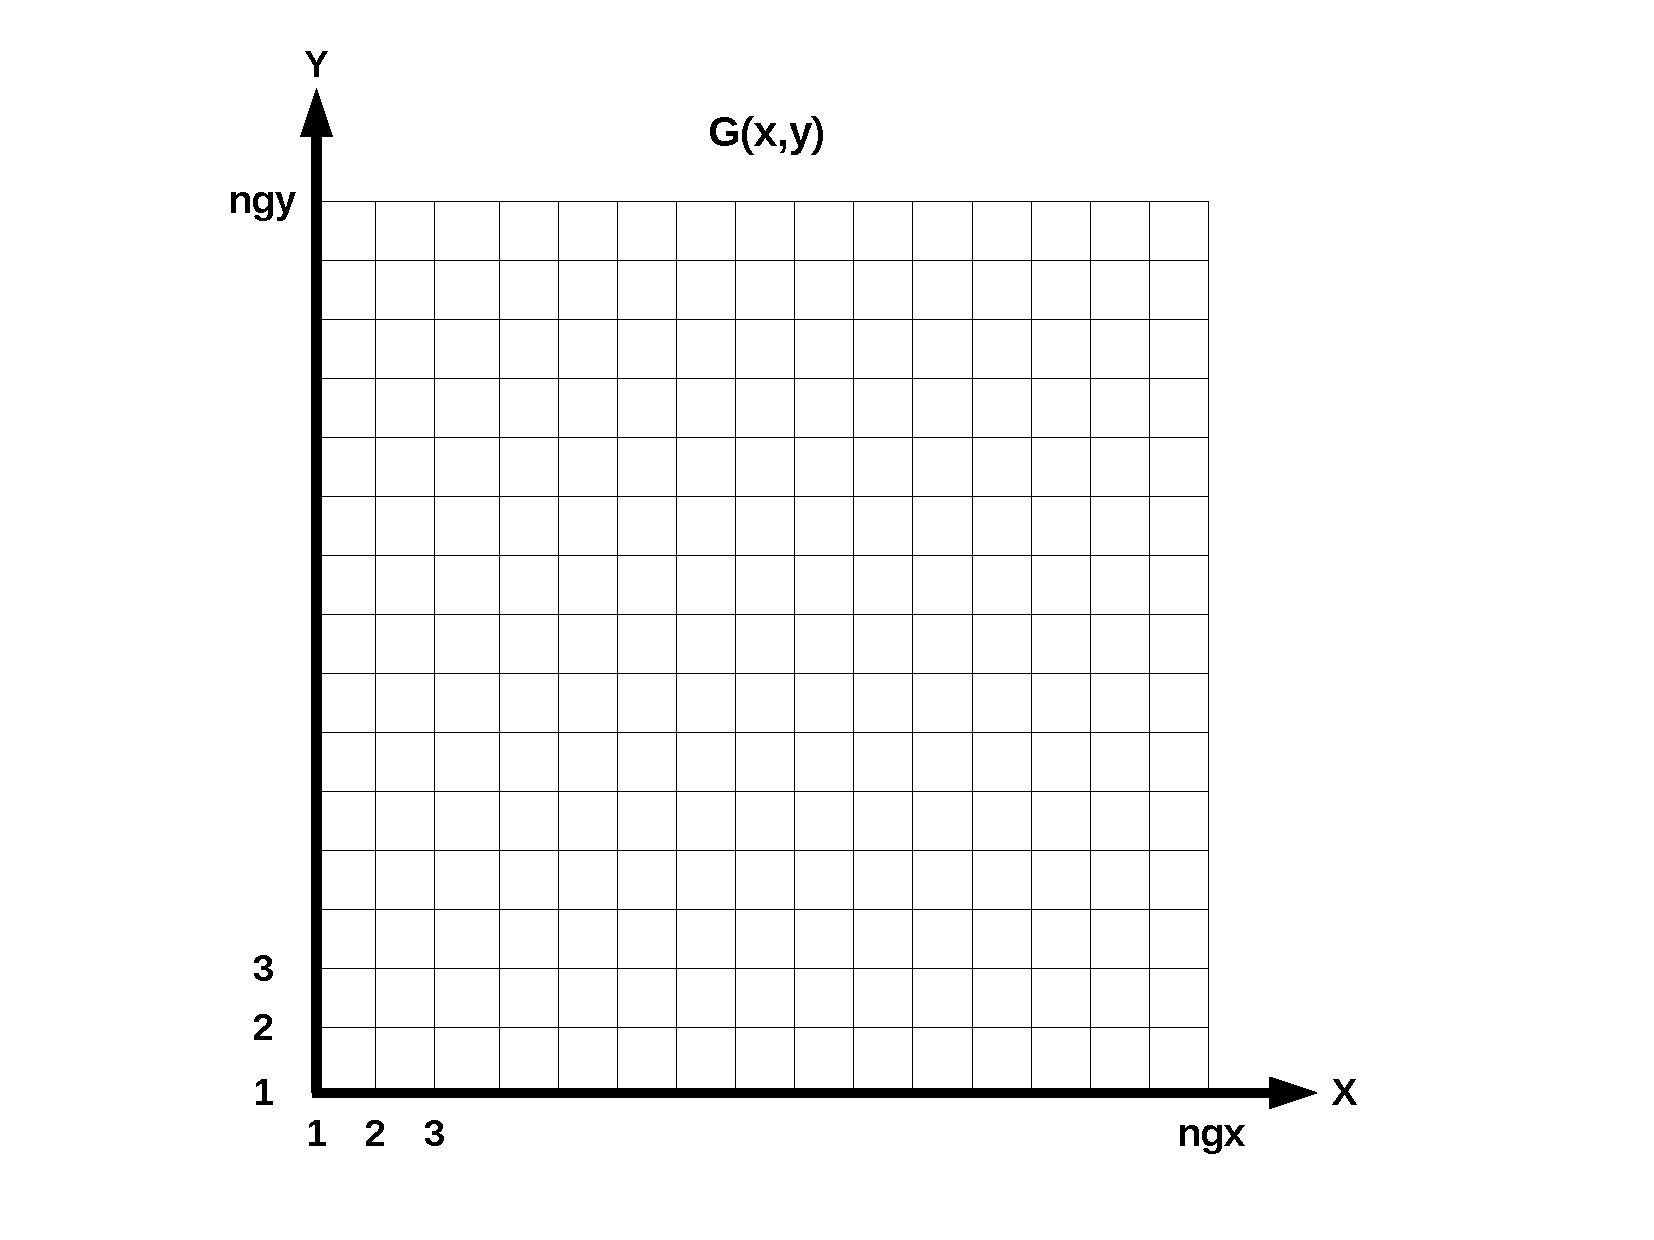
\includegraphics[height=9cm]{figures/phys_grid.pdf}
   \caption{In physical space functions $g(x,y)$ are represented on a
            regular grid with $ngx$ grid points in $x$-direction and 
            $ngy$ grid points in $y$-direction. At present in QUAD only
            the default $ngx = ngy$ is implemented.}
\end{figure}
In spectral space we have complex fields which in QUAD are either 
represented as complex $c(k_{x},k_{y})$ or as real $f(k_{x},k_{y})$ 
fields. 
\begin{figure} \label{fig_ctorspecgrid}
   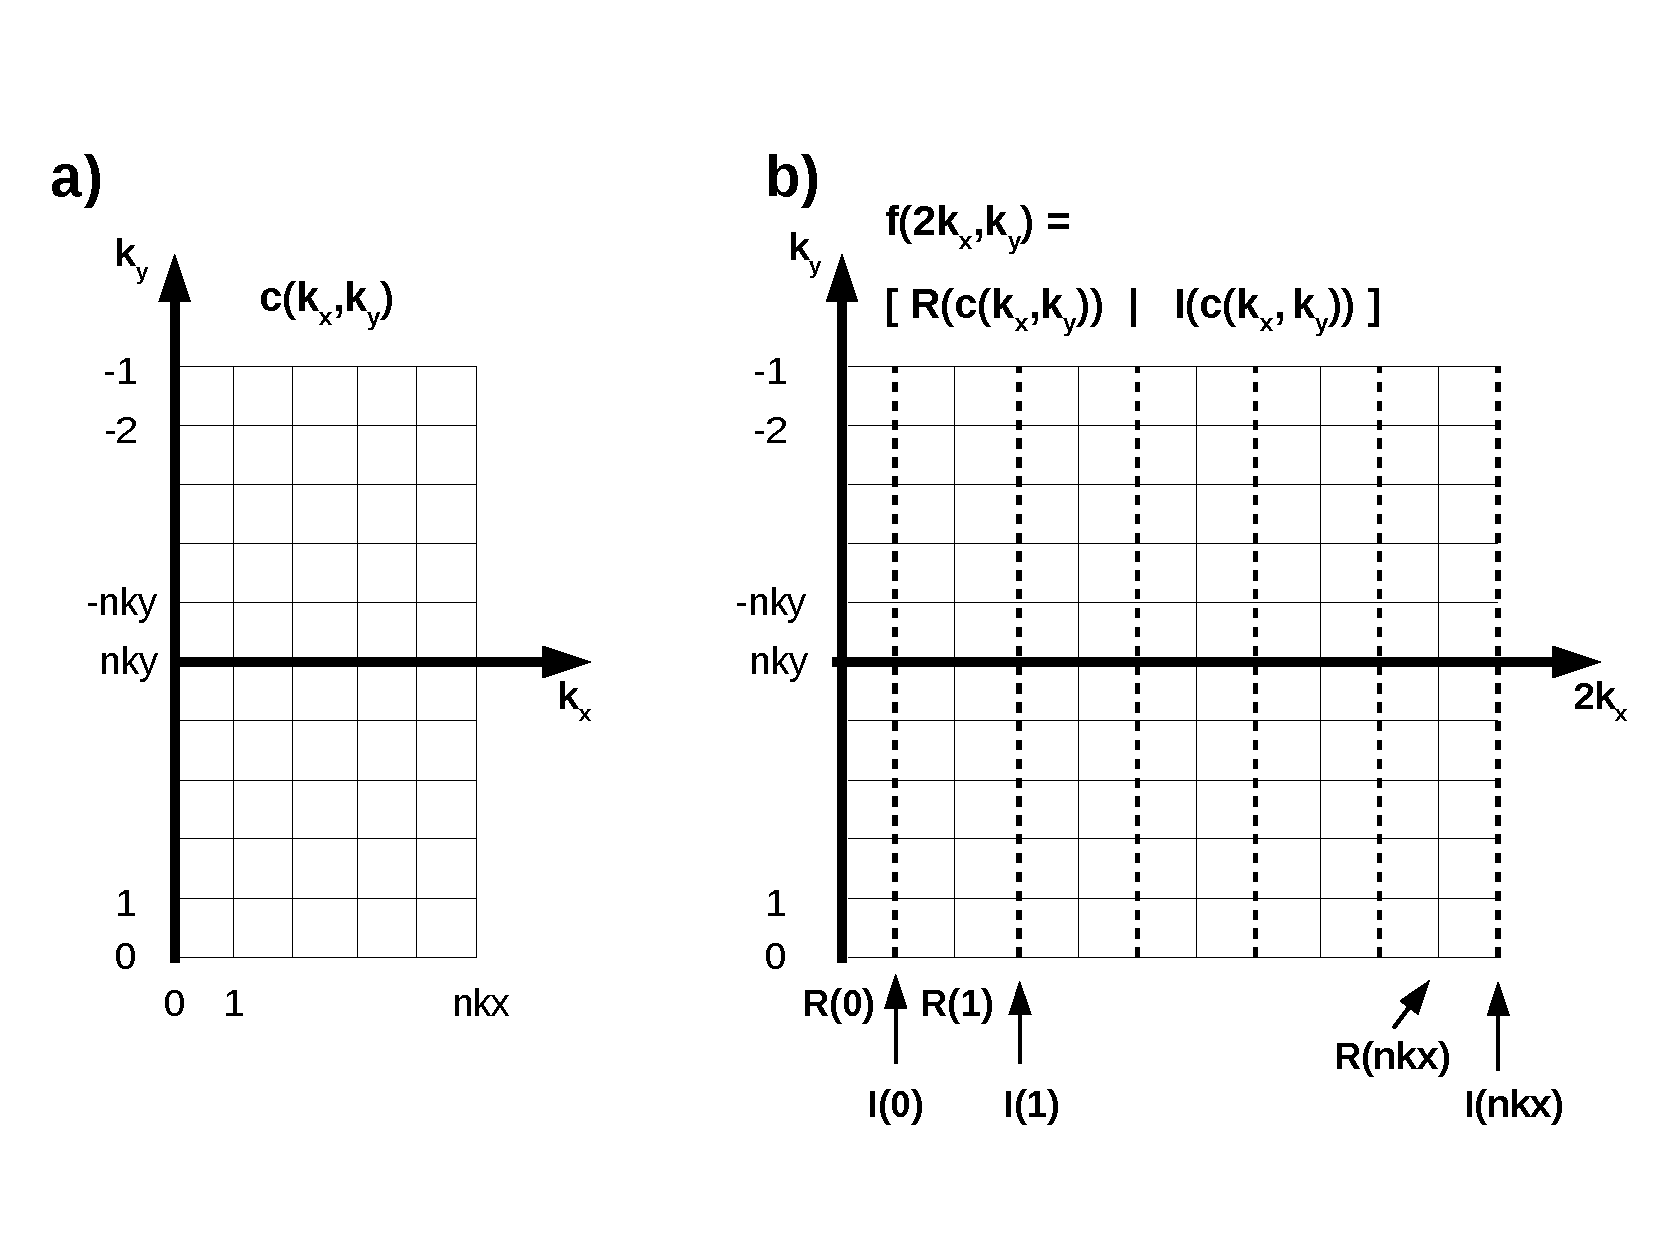
\includegraphics[height=11cm]{figures/cmplx_real_spec_grid.pdf}
   \caption{Functions in spectral space are represented either as
            complex fields $c$ or as real fields $f$ containing 
            in the first spectral coordinate $k_{x}$ the real and 
            imaginary parts of $c$ in an alternating series.}
\end{figure}
Plate (a) in figure \ref{fig_ctorspecgrid} shows the wave number
grid for the internal complex representation $c(k_{x},k_{y})$ 
of spectral fields. Due to the symmetry propreties 
\ref{eq_symfourier} it is sufficient to represent the fields only 
on half of the space wave number space, i.e.\ for the wave numbers 
\begin{equation} \label{eq_ncentwgrid}
   (k_{x},\ k_{y}) \in  
   \{\ k_{x} \in [\ 0,1,\ \dots \ nkx \ ] \ \ \mbox{and} \ \ 
   k_{y} \in [\ 0, \ \dots \ ,nky,-nky, \ \dots \ , -1 \ ] \}.
\end{equation}
As described above we use the $2/3$-truncation, so that the bounds 
$nkx$ and $nky$ are given by  
\begin{equation} \label{eq_nkxnky}
   nkx = ngx/3 \ \ \mbox{and} \ \ nky = ngy/3,
\end{equation}
where non-integer part of the division is omitted. In our example from 
above $nkx = nky = 5$. As one can see the wave-numbers 
in $y$-direction are not centered around zero. Plate (b) of 
figure \ref{fig_ctorspecgrid} shows the internal real representation 
$f(k_{x},k_{y})$ of spectral fields. In $y$-direction the spectral 
grid remains the same as in the case of the complex representation. 
In $x$-direction the number of coordinate points is doubled, even 
coordinates starting from 
$0$ hold the real part $\mathcal{R}(c(k_{x},k_{y}))$ and       
the odd coordinates starting from 1 hold the imaginary part 
$\mathcal{I}(c(k_{x},k_{y}))$ of the complex fields $c(k_{x},k_{y})$. 
This is the format QUAD reads in or writes out spectral fields.
While prescribing complex fields $c(k_{x},k_{y})$ in spectral space
to QUAD it is important to keep in mind that on the $k_{y}$-axis 
($k_{x} = 0$) values are not completely arbitrary, otherwise unphysical
complex fields in phyiscal space are created. First $c(0,0)$ has
to be zero, it represents the average of the field in physical space.
In the case of vorticity $cq$ we get $cq(0,0) = 0$. For the remaining
values $(0,k_{y})$ the symmetry properties \ref{eq_symfourier} have
to be satisfied, i.e.\ on the $k_{y}$-axis spectral fields must
satisfy the condition $c(0,k_{y}) = c^{*}(0,-k_{y})$.
\begin{figure} \label{fig_cspecgrid}
   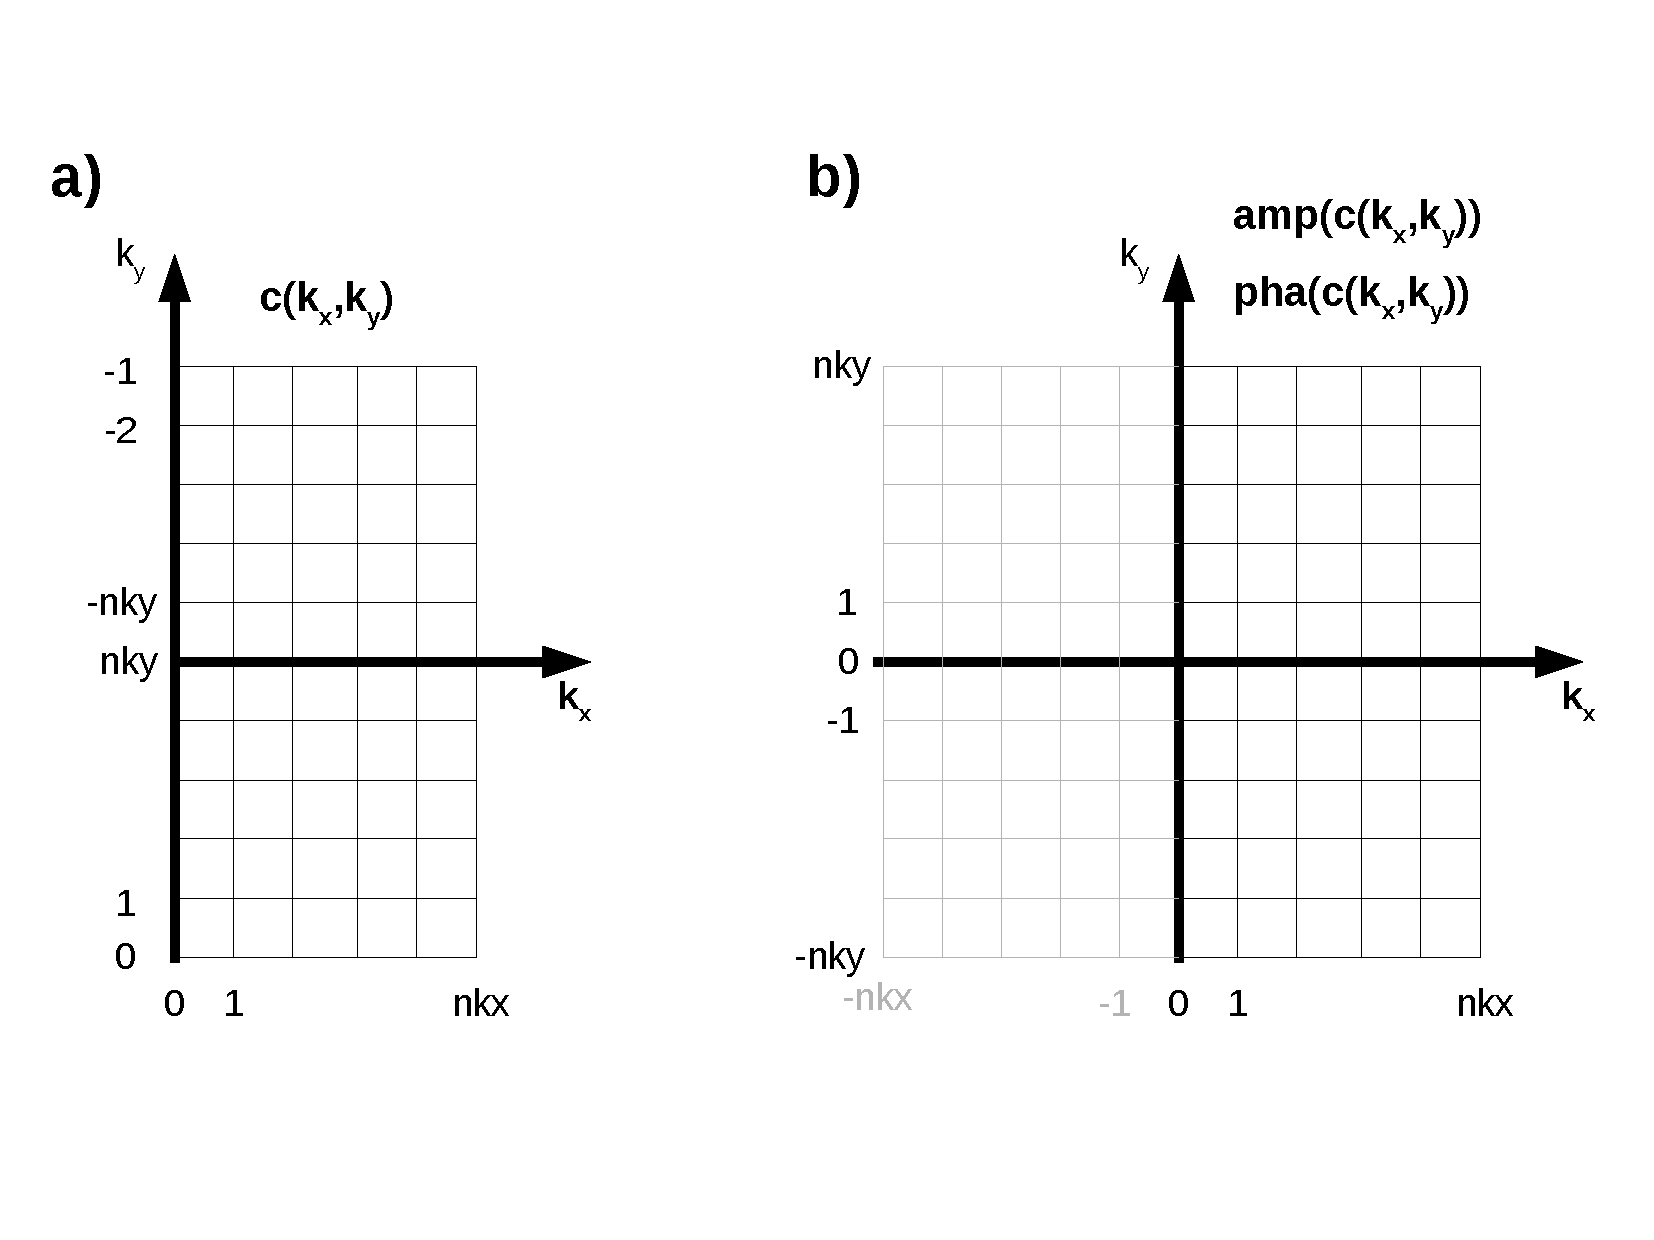
\includegraphics[height=11cm]{figures/cmplx_cent_grid.pdf}
   \caption{Internally spectral fields are given for the non-centered
            wave numbers given by equation (\ref{eq_noncentwgrid}), 
            for the visualization in the GUI the amplitudes and phases 
            of the complex spectral fields are represented on thee centered
            wave-number grid given by equation (\ref{eq_centwgrid})}
\end{figure}
In the Graphical User Interface (GUI) spectral fields are visualized on
a centerd wave-number grid
\begin{equation} \label{eq_centwgrid}
   (k_{x},\ k_{y}) \in  
   \{\ k_{x} \in [\ -nkx, \ \dots \ ,nkx \ ] 
    \ \ \mbox{and} \ \ 
       k_{y} \in [\ -nky, \ \dots \ ,nky \ ] \ \}.
\end{equation}
Visualized are the amplitudes $amp$ and phases $pha$ of the 
complex fields
\begin{equation} \label{eq_amppha}
   amp(c) = \sqrt{\mathcal{R}^{2}(c) + \mathcal{I}^{2}(c)}
   \ \ \mbox{and} \ \ 
   pha(c) = \tan^{-1}(\frac{\mathcal{I}(c)}{\mathcal{R}(c)}).
\end{equation}


